\section{mod\_jk : Relier Apache et Tomcat}
%Benoit

\subsection{Avantages}
\begin{frame}
	\begin{itemize}
		\item Apache + Tomcat sur la même machine et sur le même port
		\item Ressources statiques servies par Apache (meilleures performances)
		\item Utilisation de la configuration avancée d'Apache sur une application Java (url rewriting, htaccess...)
		\item Load balancing via le mod jk.
	\end{itemize}
\end{frame}

\subsection{Utilisation des mods}
\begin{frame}
	\frametitle{Fichiers importants}
	
	\begin{itemize}
		\item \textbf{/usr/lib/apache2/modules/mod\_x.so} :\\~~~~ Le code du module
		\item \textbf{/etc/apache2/mods-available/x.load} :\\~~~~ Instructions de chargement du module (LoadModule)
		\item \textbf{/etc/apache2/mods-available/x.conf} :\\~~~~ Configurations du module
	\end{itemize}
	
\end{frame}

\begin{frame}
	\frametitle{Utilisation d'un module}

	Fonctionnement similaire aux virtualhosts
	
	\begin{itemize}
		\item Apache lis les fichiers présents dans /etc/apache2/mods-enabled
		\item Activation d'un module : lien symbolique vers mods-available/x.load dans mods-enabled/
		\item Tâche facilitée par la commande a2enmod (apache2 enable mod)	
	\end{itemize}
	
\end{frame}

\subsection{Configuration de mod\_jk}
\begin{frame}
	\frametitle{Fonctionnement}
	
	\begin{itemize}
		\item Configuration de \og{} workers \fg{} (workers.properties)
		\item Inclusion de la configuration dans Apache (option JkWorkersFile)
		\item Redirection de certaines requêtes vers un worker (option JkMount)
	\end{itemize}
\end{frame}

\begin{frame}
	\frametitle{Fichier workers.properties}
	
	\begin{itemize}
		\item Présent dans /etc/libapache2-mod-jk/		
		\item Inclus via l'option JkWorkersFile dans mods-available/jk.conf
	\end{itemize}

	
	\begin{center}
		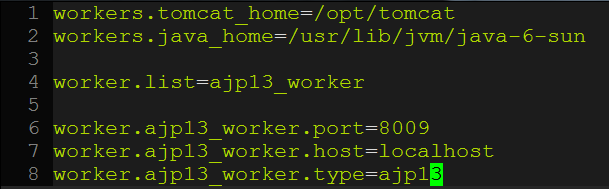
\includegraphics[scale=0.6]{Images/workers-properties.png}
	\end{center}
\end{frame}

\begin{frame}
	\frametitle{Redirection des requêtes}
	
	\begin{itemize}
		\item Option JkMount <url> <worker\_name>		
		\item En général spécifique à un virtualhost
	\end{itemize}

	\begin{center}
		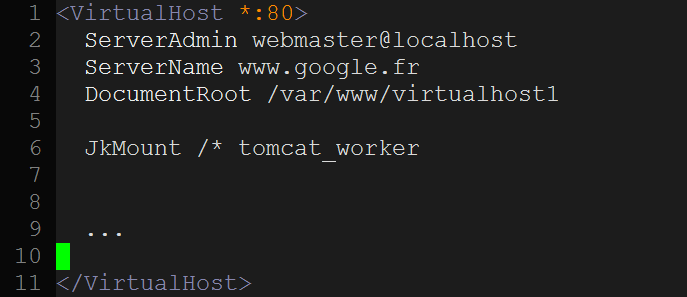
\includegraphics[scale=0.5]{Images/jkmount-example.png}
	\end{center}

\end{frame}
